\chapter{L'immunité adaptative et la vaccination}\label{ch:g12:adaptive-immunity}

En 1796, un médecin de campagne inocula au bras d'un garçon, par
scarification, le contenu d'une pustule de vaccine prélevée sur une
trayeuse, attendit six semaines, puis lui inocula la variole. Le
garçon ne tomba pas malade. Rien, dans le monde de ce médecin,
n'expliquait pourquoi~; le corps, semblait-il, avait été instruit.
Deux siècles plus tard, la variole est éteinte, et cette instruction
est comprise jusqu'aux molécules~: un ensemble de \omterm{def:g10:cells-common-unit:cell}{cellules} qui
portent, entre elles, un récepteur pour presque toute molécule pouvant
exister, qui se multiplient quand leur molécule paraît, et qui se
souviennent. Ce chapitre décrit ce système, ses deux bras, sa mémoire,
les \omterm{def:g12:adaptive-immunity:vaccine}{vaccins} bâtis sur lui --- et le virus qui le détruit.

\section{Antigènes et lymphocytes}

\begin{definition}[Antigène, lymphocyte]\label{def:g12:adaptive-immunity:antigen}
Un \emph{antigène}\index{antigène} est toute molécule que le \omterm{def:g12:innate-immunity:immunity}{système
immunitaire} adaptatif sait reconnaître~: en général une \omterm{def:g11:gene-expression:protein}{protéine} ou un
sucre de microbe, une toxine, la surface d'une \omterm{def:g10:cells-common-unit:cell}{cellule}
étrangère --- ou, par erreur, l'une de celles du corps lui-même. Les
\omterm{def:g10:cells-common-unit:cell}{cellules} qui reconnaissent sont les
\emph{lymphocytes}\index{lymphocyte}, des globules blancs fabriqués
dans la moelle osseuse et rassemblés dans les ganglions lymphatiques,
la rate et le tissu lymphoïde de l'intestin. Chaque lymphocyte porte
des milliers d'exemplaires d'un seul \emph{récepteur}, et chaque
récepteur ne lie qu'un antigène. Les \emph{lymphocytes B} mûrissent
dans la moelle et fabriqueront les \omterm{prop:g12:adaptive-immunity:antibodies}{anticorps}~; les \emph{lymphocytes
T} mûrissent dans le thymus et agissent par contact et par signaux.
\end{definition}

\begin{proposition}[Un répertoire constitué d'avance]\label{prop:g12:adaptive-immunity:repertoire}
Le récepteur de chaque \omterm{def:g12:adaptive-immunity:antigen}{lymphocyte} est assemblé, pendant que la \omterm{def:g10:cells-common-unit:cell}{cellule}
mûrit, par un réarrangement au hasard de segments de \omterm{def:g10:universal-dna:gene}{gènes}, différent
dans chaque \omterm{def:g10:cells-common-unit:cell}{cellule}. Le corps détient ainsi quelque $10^{8}$
récepteurs différents avant même d'avoir rencontré le moindre
\omterm{def:g12:adaptive-immunity:antigen}{antigène} --- assez pour que presque toute molécule trouve quelques
\omterm{def:g10:cells-common-unit:cell}{cellules} qui la lient. Les \omterm{def:g12:adaptive-immunity:antigen}{lymphocytes} dont le récepteur lie les
molécules du corps lui-même sont éliminés au cours de la maturation~;
les autres attendent, quelques \omterm{def:g10:cells-common-unit:cell}{cellules} pour chaque \omterm{def:g12:adaptive-immunity:antigen}{antigène} possible,
que leur \omterm{def:g12:adaptive-immunity:antigen}{antigène} arrive.
\end{proposition}
\admitted

\begin{omfigure}
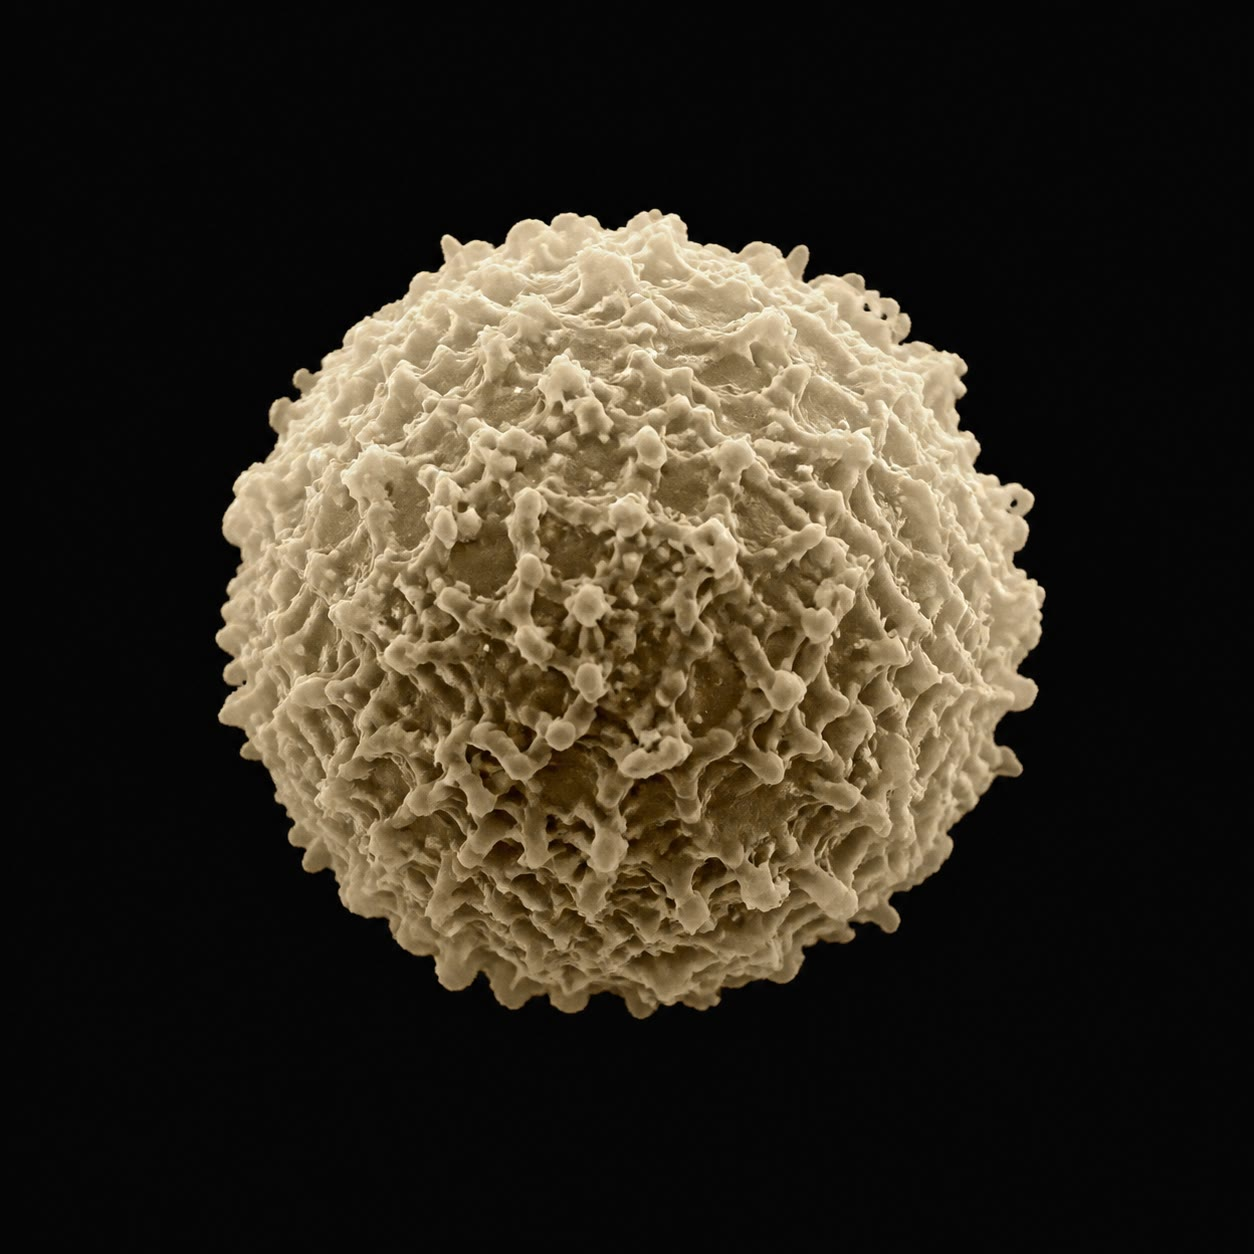
\includegraphics[width=0.36\linewidth]{images/book2/ai/g12-adaptive-lymphocyte-sem.jpg}

{\small Un \omterm{def:g12:adaptive-immunity:antigen}{lymphocyte}, sur une micrographie électronique en fausses
couleurs~: une petite \omterm{def:g10:cells-common-unit:cell}{cellule} ronde à surface rugueuse, l'une des cent
millions de sortes qui portent chacune des récepteurs pour un seul
\omterm{def:g12:adaptive-immunity:antigen}{antigène}.}
\end{omfigure}

\section{La sélection clonale}

\begin{proposition}[Sélection et amplification]\label{prop:g12:adaptive-immunity:selection}
Quand un \omterm{def:g12:adaptive-immunity:antigen}{antigène} entre, seuls répondent les \omterm{def:g12:adaptive-immunity:antigen}{lymphocytes} dont le
récepteur lui convient~: ils sont \emph{sélectionnés}, et ils se
multiplient par \omterm{def:g11:cell-cycle-mitosis:cycle}{mitose} en un clone de milliers de \omterm{def:g10:cells-common-unit:cell}{cellules} identiques
en quelques jours --- c'est la \emph{sélection
clonale}\index{sélection clonale}. Le clone se différencie ensuite~:
la plupart des \omterm{def:g10:cells-common-unit:cell}{cellules} deviennent des \emph{\omterm{def:g10:cells-common-unit:cell}{cellules} effectrices} qui
combattent l'\omterm{def:g12:adaptive-immunity:antigen}{antigène} une semaine ou deux puis meurent~; une minorité
devient des \emph{cellules mémoire}\index{cellule mémoire} à longue
vie, qui persistent des années et qui, si l'\omterm{def:g12:adaptive-immunity:antigen}{antigène} revient,
répondent plus vite et en bien plus grand nombre. La réaction est
spécifique parce que seuls les clones adaptés se multiplient~; elle
est lente la première fois parce qu'ils partent d'une poignée de
\omterm{def:g10:cells-common-unit:cell}{cellules}~; elle est rapide la seconde fois parce que les \omterm{prop:g12:adaptive-immunity:selection}{cellules
mémoire} sont déjà nombreuses.
\end{proposition}
\begin{proof}[Preuves]
Les \omterm{prop:g12:adaptive-immunity:antibodies}{anticorps} dirigés contre un \omterm{def:g12:adaptive-immunity:antigen}{antigène} donné apparaissent dans le
sang environ une semaine après une première injection, montent pendant
deux semaines puis décroissent~; une seconde injection, des mois plus
tard, produit en deux ou trois jours des \omterm{prop:g12:adaptive-immunity:antibodies}{anticorps} à dix ou cent fois
le premier maximum, qui persistent des années. Injecter un second
\omterm{def:g12:adaptive-immunity:antigen}{antigène}, sans rapport avec le premier, en même temps que la seconde
dose donne, pour cet \omterm{def:g12:adaptive-immunity:antigen}{antigène}, une réaction lente du premier type~: la
mémoire est spécifique. Des \omterm{def:g12:adaptive-immunity:antigen}{lymphocytes} prélevés sur un animal
immunisé et transférés à un animal naïf lui transmettent la mémoire~;
ceux d'un animal non immunisé ne la transmettent pas.
\end{proof}

\begin{omfigure}
\begin{tikzpicture}[font=\small, >=Stealth]
  \tikzset{lc/.style={circle, draw, thick, fill=omDef!15, minimum size=0.55cm, inner sep=0},
           sel/.style={circle, draw, thick, fill=omThm!35, minimum size=0.55cm, inner sep=0},
           mem/.style={circle, draw, thick, fill=omMeth!35, minimum size=0.55cm, inner sep=0}}
  % repertoire
  \foreach \y in {2.4,1.6,0.8,0,-0.8,-1.6} \node[lc] at (0,\y) {};
  \node[sel] at (0,0.8) {};
  \foreach \y/\a in {2.4/90,1.6/45,0.8/0,0/-45,-0.8/135,-1.6/180} \draw[thick] (0.28,\y) -- ++(\a:0.001);
  \node[anchor=south, align=center] at (0,3.0) {répertoire~: un\\ récepteur par cellule};
  % antigen
  \node[draw, fill=omThm!60, minimum size=0.25cm, inner sep=0] (ag) at (1.6,0.8) {};
  \node[anchor=north, font=\scriptsize] at (1.6,0.6) {antigène};
  \draw[->, thick] (ag) -- (0.35,0.8);
  % expansion
  \draw[->, thick] (2.4,0.8) -- (3.6,0.8) node[midway, above, font=\scriptsize, align=center] {sélection,\\ multiplication};
  \foreach \x in {4.2,4.9,5.6,6.3,7.0} \foreach \y in {1.6,0.8,0} \node[sel] at (\x,\y) {};
  \node[anchor=south, align=center] at (5.6,2.2) {clone de cellules identiques\\ (plusieurs jours)};
  % differentiation
  \draw[->, thick] (7.6,1.2) -- (8.8,1.8);
  \draw[->, thick] (7.6,0.4) -- (8.8,-0.2);
  \foreach \x in {9.4,10.1,10.8} \node[sel] at (\x,1.8) {};
  \node[anchor=west, align=left] at (11.2,1.8) {cellules effectrices~:\\ combattent,\\ puis meurent};
  \foreach \x in {9.4,10.1} \node[mem] at (\x,-0.2) {};
  \node[anchor=west, align=left] at (11.2,-0.2) {cellules mémoire~:\\ attendent\\ des années};
\end{tikzpicture}

{\small La \omterm{prop:g12:adaptive-immunity:selection}{sélection clonale}. Parmi les nombreux clones de \omterm{def:g12:adaptive-immunity:antigen}{lymphocytes}
tenus en réserve, l'\omterm{def:g12:adaptive-immunity:antigen}{antigène} sélectionne celui dont le récepteur lui
convient~; il se multiplie en quelques jours en \omterm{def:g10:cells-common-unit:cell}{cellules} effectrices
qui combattent et en \omterm{prop:g12:adaptive-immunity:selection}{cellules mémoire} qui persistent. Une seconde
rencontre trouve le clone mémoire déjà nombreux.}
\end{omfigure}

\begin{omfigure}
\begin{tikzpicture}
\begin{axis}[
  width=0.9\linewidth, height=5.8cm,
  axis x line=bottom, axis y line=left,
  xmin=0, xmax=80, ymin=0, ymax=110,
  xlabel={jours}, ylabel={anticorps dans le sang (valeur relative)},
  xlabel style={font=\small, at={(axis description cs:0.5,-0.12)}, anchor=north},
  ylabel style={font=\small},
  tick label style={font=\small}, xtick={0,10,20,30,40,50,60,70,80}, ytick={0,25,50,75,100},
  clip=false,
]
\addplot[thick, omThm, smooth] coordinates {(0,0) (5,0) (7,1) (10,4) (14,9) (18,10) (24,8) (30,5) (40,3) (50,2) (60,20) (63,60) (66,95) (70,100) (76,92) (80,85)};
\draw[->, thick] (axis cs:1,-14) -- (axis cs:1,-2); \node[font=\scriptsize, anchor=north] at (axis cs:1,-15) {première dose};
\draw[->, thick] (axis cs:56,-14) -- (axis cs:56,-2); \node[font=\scriptsize, anchor=north] at (axis cs:56,-15) {seconde dose};
\node[font=\scriptsize, anchor=south] at (axis cs:18,12) {réaction primaire};
\node[font=\scriptsize, anchor=east] at (axis cs:68,100) {réaction secondaire};
\end{axis}
\end{tikzpicture}

{\small Les \omterm{prop:g12:adaptive-immunity:antibodies}{anticorps} après deux doses du même \omterm{def:g12:adaptive-immunity:antigen}{antigène}. La réaction
primaire commence après une semaine et reste modeste~; la secondaire,
issue des \omterm{prop:g12:adaptive-immunity:selection}{cellules mémoire}, commence en quelques jours et atteint dix
fois le niveau --- c'est le principe de la dose de rappel.}
\end{omfigure}

\section{Deux bras~: les anticorps et les cellules tueuses}

\begin{proposition}[Les lymphocytes B et les anticorps]\label{prop:g12:adaptive-immunity:antibodies}
Un clone B sélectionné se différencie en \emph{plasmocytes}, des
usines qui sécrètent des milliers d'\emph{anticorps}\index{anticorps}
par seconde~: des copies solubles du récepteur du clone, des \omterm{def:g10:chemistry-of-life:families}{protéines}
en forme d'Y dont les deux bras lient chacun l'\omterm{def:g12:adaptive-immunity:antigen}{antigène}. Les \omterm{prop:g12:adaptive-immunity:antibodies}{anticorps}
ne tuent pas~; ils \emph{marquent}. Liés à un virus ou à une toxine,
ils l'empêchent d'entrer dans les \omterm{def:g10:cells-common-unit:cell}{cellules} ou d'agir~; liés à une
bactérie, ils l'enrobent, et c'est cet enrobage que les \omterm{def:g12:innate-immunity:phagocytosis}{phagocytes} du
\cref{ch:g12:innate-immunity} saisissent le mieux. Les \omterm{def:g12:adaptive-immunity:antigen}{antigènes}
pontés par de nombreux \omterm{prop:g12:adaptive-immunity:antibodies}{anticorps} s'agrègent en \emph{complexes
immuns}, que la \omterm{def:g12:innate-immunity:phagocytosis}{phagocytose} élimine. C'est le bras dirigé contre les
intrus présents dans le sang et les liquides.
\end{proposition}
\admitted

\begin{omfigure}
\begin{tikzpicture}[font=\small, line cap=round, >=Stealth]
  % antibody Y
  \draw[line width=5pt, omDef!70] (0,-1.6) -- (0,0);
  \draw[line width=5pt, omDef!70] (0,0) -- (-1.1,1.3);
  \draw[line width=5pt, omDef!70] (0,0) -- (1.1,1.3);
  \draw[line width=3pt, omDef!35] (0.25,-1.6) -- (0.25,0.05) -- (1.3,1.1);
  \draw[line width=3pt, omDef!35] (-0.25,-1.6) -- (-0.25,0.05) -- (-1.3,1.1);
  \node[draw, fill=omThm!60, minimum size=0.28cm, inner sep=0, rotate=40] at (-1.35,1.6) {};
  \node[draw, fill=omThm!60, minimum size=0.28cm, inner sep=0, rotate=-40] at (1.35,1.6) {};
  \node[anchor=west, align=left] at (1.9,1.6) {antigène lié à l'extrémité\\ de chaque bras};
  \node[anchor=west, align=left] at (1.9,-1.2) {tige~: saisie par les\\ phagocytes};
  \draw[->] (1.85,-1.2) -- (0.35,-1.2);
  \node[anchor=north, align=center] at (0,-1.9) {un anticorps~: deux bras,\\ une seule spécificité};
  % complex
  \begin{scope}[xshift=8.6cm]
    \foreach \x/\y in {0/0, 1.2/0.6, 0.4/1.3, 1.6/-0.5, -0.6/0.9}
      \node[draw, fill=omThm!60, minimum size=0.28cm, inner sep=0] at (\x,\y) {};
    \foreach \a/\b in {0/0.6, 0.6/1.15, 1.15/0.65, 0.65/1.45, 1.45/-0.05, -0.05/0.75, 0.75/-0.6}
      \draw[line width=2.5pt, omDef!70] (\a,\b) -- ++(0.35,-0.25);
    \draw[line width=2.5pt, omDef!70] (0.1,0.05) -- (1.1,0.55); \draw[line width=2.5pt, omDef!70] (0.5,1.2) -- (1.15,0.65);
    \draw[line width=2.5pt, omDef!70] (-0.5,0.85) -- (0.3,1.25); \draw[line width=2.5pt, omDef!70] (1.25,0.5) -- (1.55,-0.4);
    \draw[line width=2.5pt, omDef!70] (0.05,-0.05) -- (1.5,-0.45);
    \node[anchor=north, align=center] at (0.5,-1.4) {complexe immun~: antigènes\\ pontés, prêts pour la phagocytose};
  \end{scope}
\end{tikzpicture}

{\small Un \omterm{prop:g12:adaptive-immunity:antibodies}{anticorps} et ce qu'il fait. Les deux bras lient
l'\omterm{def:g12:adaptive-immunity:antigen}{antigène}~; la tige est reconnue par les \omterm{def:g12:innate-immunity:phagocytosis}{phagocytes}. De nombreux
\omterm{prop:g12:adaptive-immunity:antibodies}{anticorps} liant de nombreux \omterm{def:g12:adaptive-immunity:antigen}{antigènes} forment un complexe qu'un
\omterm{def:g12:innate-immunity:phagocytosis}{phagocyte} engloutit d'un seul coup.}
\end{omfigure}

\begin{proposition}[Les lymphocytes T]\label{prop:g12:adaptive-immunity:tcells}
Les \omterm{def:g12:adaptive-immunity:antigen}{lymphocytes} T ne reconnaissent l'\omterm{def:g12:adaptive-immunity:antigen}{antigène} que sous forme de
fragments exposés à la surface d'une autre \omterm{def:g10:cells-common-unit:cell}{cellule}
(\cref{ch:g12:innate-immunity}). Il en existe deux sortes~:
\begin{itemize}
  \item Les \emph{lymphocytes T auxiliaires}\index{lymphocyte T auxiliaire}
        sont activés par les \omterm{prop:g12:innate-immunity:handover}{cellules dendritiques} qui apportent
        l'\omterm{def:g12:adaptive-immunity:antigen}{antigène} au ganglion lymphatique~; une fois sélectionnés et
        multipliés, ils sécrètent des cytokines qui autorisent et
        amplifient la réaction des \omterm{def:g12:adaptive-immunity:antigen}{lymphocytes} B et des autres
        \omterm{def:g12:adaptive-immunity:antigen}{lymphocytes} T. Ce sont les coordinateurs~; sans eux, presque
        aucune réaction adaptative n'a lieu.
  \item Les \emph{\omterm{def:g12:adaptive-immunity:antigen}{lymphocytes} T cytotoxiques} reconnaissent les
        fragments d'un virus (ou d'une \omterm{def:g11:gene-expression:protein}{protéine} tumorale) exposés par
        une \omterm{def:g10:cells-common-unit:cell}{cellule} infectée, et tuent cette \omterm{def:g10:cells-common-unit:cell}{cellule} par contact,
        avant que le virus qu'elle abrite ait pu se multiplier. C'est
        le bras dirigé contre les intrus cachés dans les \omterm{def:g10:cells-common-unit:cell}{cellules}, là
        où les \omterm{prop:g12:adaptive-immunity:antibodies}{anticorps} ne peuvent pas atteindre.
\end{itemize}
\end{proposition}
\admitted

\begin{omfigure}
\begin{tikzpicture}[font=\small, >=Stealth,
  b/.style={draw, rounded corners, align=center, text width=2.8cm, minimum height=1.1cm}]
  \node[b, fill=omProp!15] (dc) at (0,0) {cellule dendritique~:\\ présente des fragments\\ d'antigène};
  \node[b, fill=omThm!15, text width=3.0cm] (th) at (4.4,0) {lymphocytes T auxiliaires~:\\ sélectionnés, multipliés,\\ sécrètent des cytokines};
  \node[b, fill=omDef!12] (bc) at (9.2,1.6) {lymphocytes B~: plasmocytes,\\ anticorps};
  \node[b, fill=omDef!12] (tc) at (9.2,-1.6) {lymphocytes T cytotoxiques~:\\ tuent les cellules infectées};
  \node[b, fill=omMeth!15, text width=2.4cm] (mem) at (13.2,0) {cellules mémoire\\ des trois};
  \draw[->, thick] (dc) -- (th);
  \draw[->, thick] (th) -- node[above, sloped, font=\scriptsize] {cytokines} (bc);
  \draw[->, thick] (th) -- node[below, sloped, font=\scriptsize] {cytokines} (tc);
  \draw[->, thick] (bc) -- (mem); \draw[->, thick] (tc) -- (mem); \draw[->, thick] (th) -- (mem);
\end{tikzpicture}

{\small L'organisation de la réaction adaptative. Le rapport de la
\omterm{prop:g12:innate-immunity:handover}{cellule dendritique} active les \omterm{prop:g12:adaptive-immunity:tcells}{lymphocytes T auxiliaires}, dont les
cytokines autorisent les \omterm{def:g12:adaptive-immunity:antigen}{lymphocytes} B à fabriquer des \omterm{prop:g12:adaptive-immunity:antibodies}{anticorps} et
les \omterm{def:g12:adaptive-immunity:antigen}{lymphocytes} T cytotoxiques à tuer~; chaque bras laisse derrière
lui des \omterm{prop:g12:adaptive-immunity:selection}{cellules mémoire}.}
\end{omfigure}

\begin{example}[Un virus, rencontré deux fois]\label{ex:g12:adaptive-immunity:virus}
Première grippe~: le virus se multiplie trois jours avant que la
réaction adaptative soit prête~; au jour 7, des \omterm{def:g12:adaptive-immunity:antigen}{lymphocytes} T
cytotoxiques tuent les \omterm{def:g10:cells-common-unit:cell}{cellules} infectées des voies respiratoires et
des \omterm{prop:g12:adaptive-immunity:antibodies}{anticorps} neutralisent le virus libre~; au jour 10, la personne se
rétablit, avec des \omterm{prop:g12:adaptive-immunity:selection}{cellules mémoire} des deux sortes. La même souche un
an plus tard~: des \omterm{prop:g12:adaptive-immunity:antibodies}{anticorps} déjà présents dans le sang bloquent
l'essentiel du virus à l'entrée, les \omterm{prop:g12:adaptive-immunity:selection}{cellules mémoire} se multiplient
en deux jours, et l'infection est finie avant d'avoir été remarquée.
Une souche différente, dont les \omterm{def:g10:chemistry-of-life:families}{protéines} de surface ont muté, échappe
aux \omterm{prop:g12:adaptive-immunity:antibodies}{anticorps} --- c'est pourquoi le \omterm{def:g12:adaptive-immunity:vaccine}{vaccin} est refait chaque année.
\end{example}

\section{La vaccination}

\begin{definition}[Vaccin]\label{def:g12:adaptive-immunity:vaccine}
Un \emph{vaccin}\index{vaccin} est une préparation qui provoque une
réaction adaptative primaire, et donc une mémoire, contre un agent
pathogène sans en causer la maladie~: l'agent atténué (rougeole,
tuberculose), tué (poliomyélite injectable), réduit à l'une de ses
\omterm{def:g10:chemistry-of-life:families}{protéines} ou à une toxine inactivée (tétanos, hépatite B), ou, tout
récemment, aux instructions permettant à la \omterm{def:g10:cells-common-unit:cell}{cellule} de fabriquer cette
\omterm{def:g11:gene-expression:protein}{protéine}. Un \emph{adjuvant} ajouté à la préparation provoque la
petite inflammation sans laquelle les \omterm{prop:g12:innate-immunity:handover}{cellules dendritiques} ne
porteraient pas l'\omterm{def:g12:adaptive-immunity:antigen}{antigène} au ganglion lymphatique. Les doses de
rappel transforment la réaction primaire en réaction secondaire et
prolongent la mémoire de plusieurs décennies.
\end{definition}

\begin{omfigure}
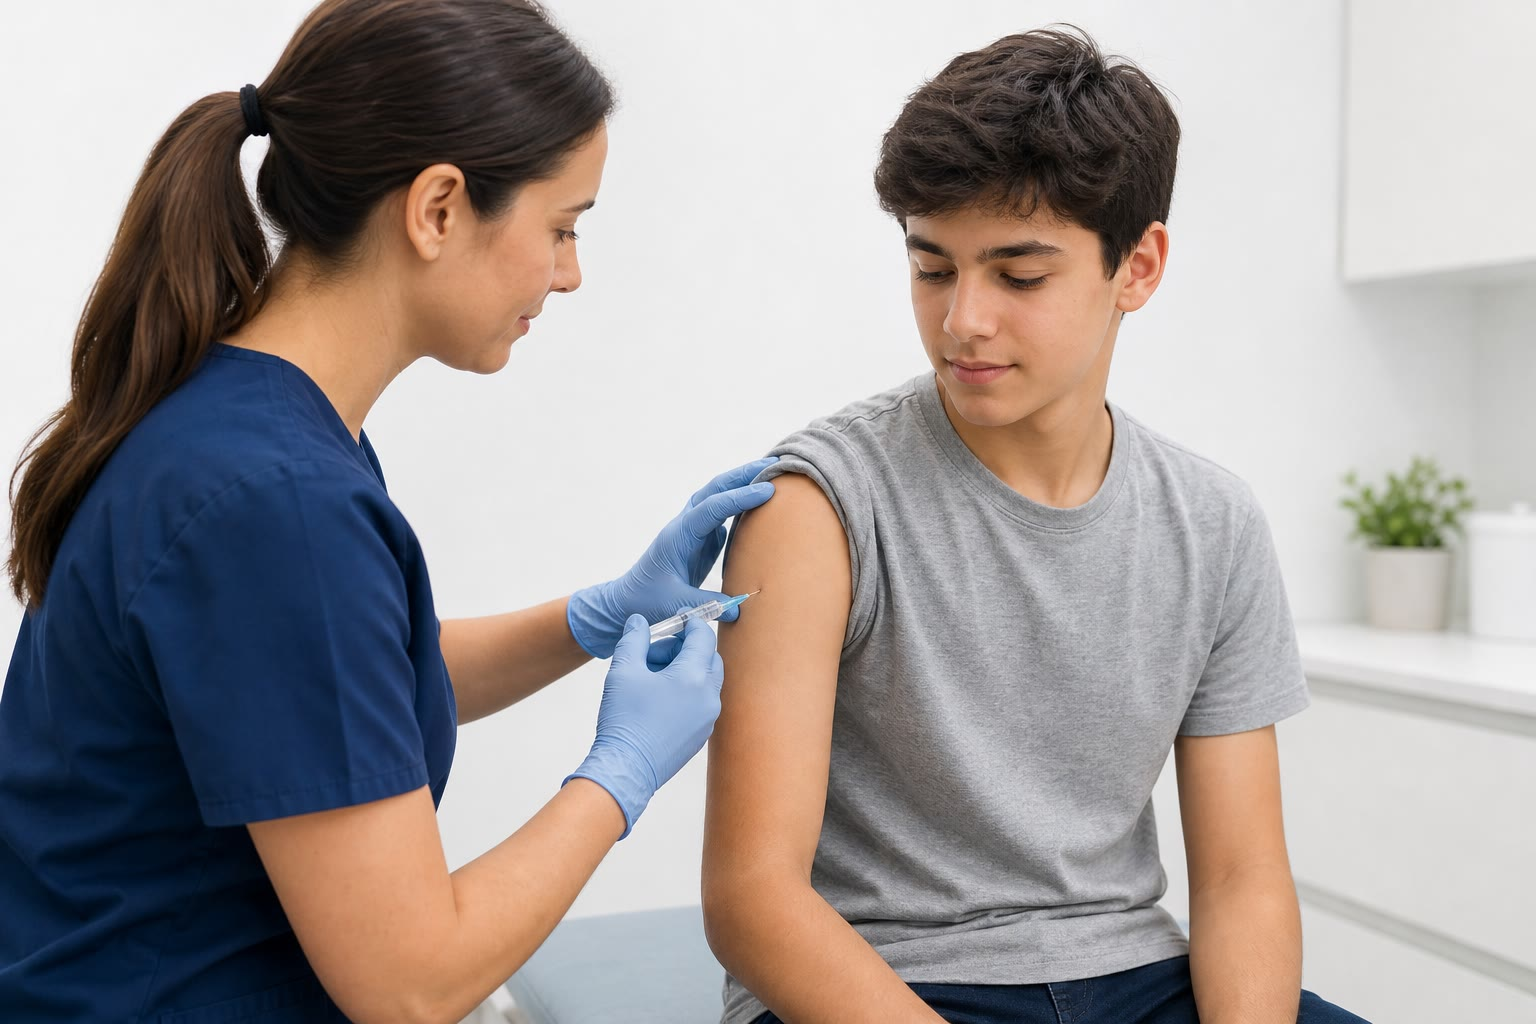
\includegraphics[width=0.56\linewidth]{images/book2/ai/g12-adaptive-vaccination.jpg}

{\small Une vaccination~: un \omterm{def:g12:adaptive-immunity:antigen}{antigène} délivré dans le bras, avec un
adjuvant pour susciter une inflammation locale. En quelques semaines,
les ganglions lymphatiques détiennent des \omterm{prop:g12:adaptive-immunity:selection}{cellules mémoire} contre une
maladie que la personne n'a jamais eue.}
\end{omfigure}

\begin{omfigure}
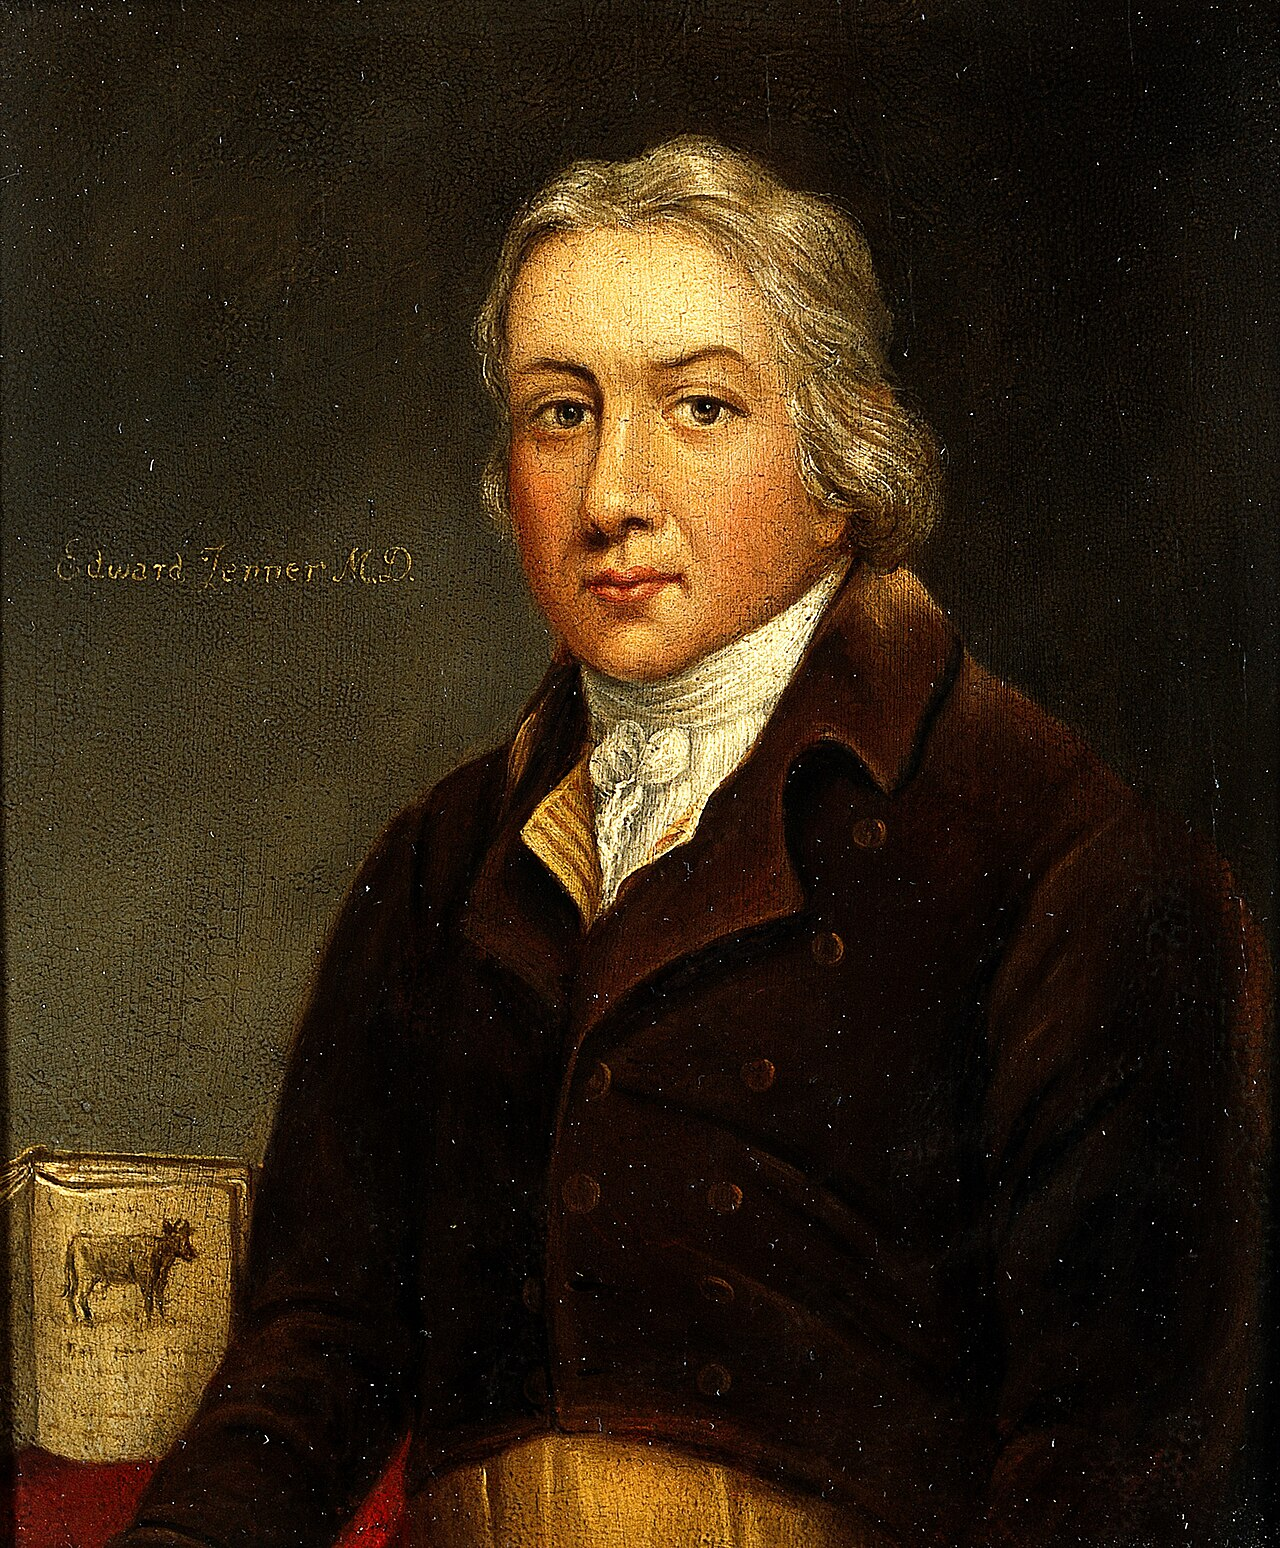
\includegraphics[width=0.34\linewidth]{images/book1/jenner.jpg}

{\small Edward Jenner, qui montra en 1796 que l'inoculation de la
vaccine protégeait de la variole --- la vaccination, avant qu'aucun de
ses mécanismes ne soit connu. Peinture à l'huile, Wellcome Collection,
CC BY 4.0.}
\end{omfigure}

\begin{proposition}[Protéger le groupe]\label{prop:g12:adaptive-immunity:herd}
Une personne vaccinée est protégée~; une \omterm{def:g12:selection-drift-speciation:population}{population} vaccinée protège
aussi ses membres non vaccinés. Une personne infectée transmet une
maladie, en moyenne, à $R_0$ autres personnes dans une \omterm{def:g12:selection-drift-speciation:population}{population} sans
immunité (environ 15 pour la rougeole, 2 à 3 pour la grippe)~; si une
fraction $v$ est immunisée, seuls $R_0(1 - v)$ de ces contacts peuvent
être infectés, et la maladie recule quand ce nombre tombe au-dessous
de 1 --- c'est-à-dire quand
\[
v > 1 - \frac{1}{R_0}.
\]
Pour la rougeole, 93\% de la \omterm{def:g12:selection-drift-speciation:population}{population} doit être immunisée pour
protéger aussi les nourrissons trop jeunes pour le \omterm{def:g12:adaptive-immunity:vaccine}{vaccin} et les
personnes qui ne peuvent pas le recevoir~; pour la grippe, environ
60\%. Cette \emph{immunité collective}\index{immunité collective} est
ce qui fait de la vaccination un acte collectif.
\end{proposition}
\admitted

\begin{omfigure}
\begin{tikzpicture}
\begin{axis}[
  width=0.84\linewidth, height=5.4cm,
  axis x line=bottom, axis y line=left,
  xmin=0, xmax=20, ymin=0, ymax=100,
  xlabel={$R_0$ de la maladie}, ylabel={fraction vaccinée nécessaire (\%)},
  xlabel style={font=\small, at={(axis description cs:0.5,-0.12)}, anchor=north},
  ylabel style={font=\small},
  tick label style={font=\small}, xtick={0,5,10,15,20}, ytick={0,25,50,75,100},
  clip=false,
]
\addplot[thick, omThm, domain=1:20, samples=100] {100*(1-1/x)};
\draw[dashed, gray] (axis cs:2.5,0) -- (axis cs:2.5,60); \node[font=\scriptsize, anchor=west] at (axis cs:2.9,48) {grippe};
\draw[dashed, gray] (axis cs:6,0) -- (axis cs:6,83); \node[font=\scriptsize, anchor=south] at (axis cs:6,85) {poliomyélite};
\draw[dashed, gray] (axis cs:15,0) -- (axis cs:15,93); \node[font=\scriptsize, anchor=south] at (axis cs:15,95) {rougeole};
\end{axis}
\end{tikzpicture}

{\small La fraction d'une \omterm{def:g12:selection-drift-speciation:population}{population} qui doit être immunisée pour
arrêter la propagation d'une maladie, en fonction du $R_0$ de
celle-ci. Plus la maladie est contagieuse, plus la couverture doit
approcher la totalité.}
\end{omfigure}

\section{Quand le coordinateur est détruit}

\begin{proposition}[Le VIH et le sida]\label{prop:g12:adaptive-immunity:hiv}
Le virus de l'immunodéficience humaine, le VIH, infecte les
\omterm{prop:g12:adaptive-immunity:tcells}{lymphocytes T auxiliaires}, en entrant par le récepteur même qui les
caractérise, et s'y multiplie. Pendant des années, le \omterm{def:g12:innate-immunity:immunity}{système
immunitaire} tue les \omterm{def:g10:cells-common-unit:cell}{cellules} infectées et fabrique des
\omterm{prop:g12:adaptive-immunity:antibodies}{anticorps} --- la personne est \emph{séropositive}, et
contagieuse --- tandis que le virus, qui mute sans cesse, échappe à
chaque réaction et épuise lentement les \omterm{def:g12:adaptive-immunity:antigen}{lymphocytes} auxiliaires. Quand
leur nombre tombe au-dessous du cinquième environ de la normale, la
réaction adaptative ne peut plus être coordonnée~: c'est le
\emph{sida}\index{sida}, où des infections qu'un corps sain élimine
sans s'en apercevoir --- un champignon de la bouche, un parasite bénin
des poumons --- deviennent mortelles, et où des \omterm{def:g11:cancer:cancer}{cancers} rares
apparaissent. Des médicaments antiviraux bloquent les \omterm{def:g11:enzymes-and-phenotype:enzyme}{enzymes} du
virus, restaurent les \omterm{def:g12:adaptive-immunity:antigen}{lymphocytes} auxiliaires et, pris à vie,
tiennent la maladie à distance et arrêtent la transmission~; il n'y a
pas encore de \omterm{def:g12:adaptive-immunity:vaccine}{vaccin}, ni de guérison.
\end{proposition}
\admitted

\begin{omfigure}
\begin{tikzpicture}
\begin{axis}[
  width=0.9\linewidth, height=6cm,
  axis x line=bottom, axis y line=left,
  xmin=0, xmax=11, ymin=0, ymax=1200,
  xlabel={années après l'infection (sans traitement)}, ylabel={lymphocytes T auxiliaires par \unit{\micro L} de sang},
  xlabel style={font=\small, at={(axis description cs:0.5,-0.12)}, anchor=north},
  ylabel style={font=\small},
  tick label style={font=\small}, xtick={0,2,4,6,8,10}, ytick={0,200,400,600,800,1000},
  clip=false,
]
\addplot[thick, omDef, smooth] coordinates {(0,1000) (0.2,550) (0.5,800) (1,750) (3,650) (5,520) (7,380) (8,280) (9,180) (10,90) (11,40)};
\addplot[thick, omThm, dashed, smooth] coordinates {(0,50) (0.15,900) (0.4,300) (1,150) (3,170) (5,220) (7,320) (8,450) (9,650) (10,900) (11,1100)};
\draw[dashed, gray] (axis cs:0,200) -- (axis cs:11,200);
\node[font=\scriptsize, gray, anchor=north] at (axis cs:5.5,190) {seuil du sida};
\node[font=\scriptsize, omDef, anchor=south] at (axis cs:4,680) {lymphocytes T auxiliaires};
\node[font=\scriptsize, omThm, anchor=north] at (axis cs:2.4,130) {virus dans le sang (valeur relative)};
\end{axis}
\end{tikzpicture}

{\small L'évolution d'une infection à VIH non traitée (moyenne
arrondie). Après une première flambée, le virus est contenu pendant
des années par la réaction immunitaire tandis que les \omterm{prop:g12:adaptive-immunity:tcells}{lymphocytes T
auxiliaires} déclinent~; au-dessous de 200 par microlitre environ, la
réaction s'effondre, le virus repart, et les infections opportunistes
commencent.}
\end{omfigure}

\begin{omfigure}
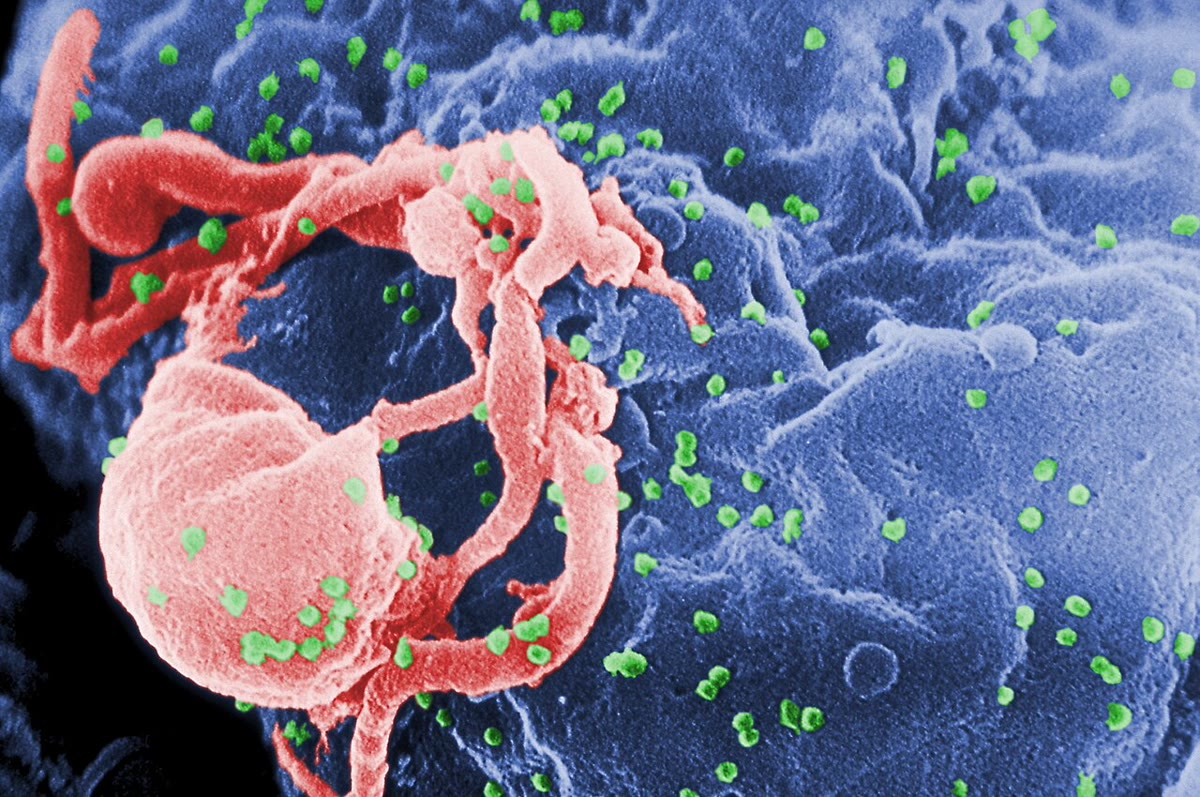
\includegraphics[width=0.6\linewidth]{images/book2/hiv-budding.jpg}

{\small Des particules de VIH (en vert) bourgeonnant à la surface d'un \omterm{def:g12:adaptive-immunity:antigen}{lymphocyte} infecté, sur une micrographie électronique en fausses couleurs. Chaque particule porte des copies du génome du virus, et parmi elles les mutants que la réaction suivante ne reconnaîtra pas. Micrographie de C.~Goldsmith, CDC, domaine public.}
\end{omfigure}

\begin{method}[Lire une réaction immunitaire]\label{met:g12:adaptive-immunity:read}
\begin{enumerate}
  \item Repérer l'\omterm{def:g12:adaptive-immunity:antigen}{antigène} et sa localisation~: libre dans les
        liquides (les \omterm{prop:g12:adaptive-immunity:antibodies}{anticorps} agissent) ou à l'intérieur des
        \omterm{def:g10:cells-common-unit:cell}{cellules} (les \omterm{def:g12:adaptive-immunity:antigen}{lymphocytes} T cytotoxiques agissent).
  \item Lire le calendrier~: une semaine jusqu'au maximum signale une
        réaction primaire, quelques jours signalent la mémoire.
  \item Lire la spécificité~: une réaction à un \omterm{def:g12:adaptive-immunity:antigen}{antigène} laisse
        intacte la réaction à un autre.
  \item Situer les \omterm{prop:g12:adaptive-immunity:tcells}{lymphocytes T auxiliaires}~: sans eux, rien ne se
        passe, ce que le \omterm{prop:g12:adaptive-immunity:hiv}{sida} démontre.
  \item Pour un \omterm{def:g12:adaptive-immunity:vaccine}{vaccin}, nommer la forme de l'\omterm{def:g12:adaptive-immunity:antigen}{antigène}, l'adjuvant, le
        nombre de doses, et la fraction de la \omterm{def:g12:selection-drift-speciation:population}{population} nécessaire.
\end{enumerate}
\end{method}

\begin{remark}[La sélection, une fois de plus]\label{rem:g12:adaptive-immunity:selection}
Le \omterm{def:g12:innate-immunity:immunity}{système immunitaire} adaptatif est darwinien~: une \omterm{def:g12:selection-drift-speciation:population}{population} de
\omterm{def:g10:cells-common-unit:cell}{cellules} à récepteurs aléatoires, dont le milieu ---
l'\omterm{def:g12:adaptive-immunity:antigen}{antigène} --- sélectionne quelques-unes pour qu'elles se multiplient,
et dont les descendantes héritent du récepteur gagnant. Il déroule le
processus du \cref{ch:g12:selection-drift-speciation} à l'intérieur
d'un seul corps en une semaine et, par la mémoire, en garde les
résultats toute une vie. C'est aussi la raison pour laquelle le
\omterm{def:g12:innate-immunity:immunity}{système immunitaire} peut être instruit, ce que fait un \omterm{def:g12:adaptive-immunity:vaccine}{vaccin}, et pour
laquelle un virus qui mute plus vite que le système ne
sélectionne --- le VIH, la grippe --- est si difficile à vaincre.
\end{remark}

\section{Exercices}

\begin{exercise}[$\star$]\label{exo:g12:adaptive-immunity:1}
Définir l'\omterm{def:g12:adaptive-immunity:antigen}{antigène} et le \omterm{def:g12:adaptive-immunity:antigen}{lymphocyte}, et dire ce qui fait la
spécificité de chaque \omterm{def:g12:adaptive-immunity:antigen}{lymphocyte}.
\end{exercise}

\begin{exercise}[$\star$]\label{exo:g12:adaptive-immunity:2}
Décrire la \omterm{prop:g12:adaptive-immunity:selection}{sélection clonale} en quatre étapes.
\end{exercise}

\begin{exercise}[$\star$]\label{exo:g12:adaptive-immunity:3}
Qu'est-ce qu'un \omterm{prop:g12:adaptive-immunity:antibodies}{anticorps}, que lie-t-il, et que fait-il à une
bactérie~?
\end{exercise}

\begin{exercise}[$\star$]\label{exo:g12:adaptive-immunity:4}
Donner les rôles des \omterm{prop:g12:adaptive-immunity:tcells}{lymphocytes T auxiliaires} et des \omterm{def:g12:adaptive-immunity:antigen}{lymphocytes} T
cytotoxiques.
\end{exercise}

\begin{exercise}[$\star$]\label{exo:g12:adaptive-immunity:5}
Que contient un \omterm{def:g12:adaptive-immunity:vaccine}{vaccin}, et pourquoi fonctionne-t-il~?
\end{exercise}

\begin{exercise}[$\star\star$]\label{exo:g12:adaptive-immunity:6}
D'après la figure des \omterm{prop:g12:adaptive-immunity:antibodies}{anticorps}, comparer le délai, le maximum et la
durée des réactions primaire et secondaire.
\end{exercise}

\begin{exercise}[$\star\star$]\label{exo:g12:adaptive-immunity:7}
Une seconde injection de l'\omterm{def:g12:adaptive-immunity:antigen}{antigène} A en même temps qu'une première
injection de l'\omterm{def:g12:adaptive-immunity:antigen}{antigène} B donne une réaction forte et rapide à A et
une réaction lente et faible à B. Que montre ce fait~?
\end{exercise}

\begin{exercise}[$\star\star$]\label{exo:g12:adaptive-immunity:8}
Pourquoi les \omterm{prop:g12:adaptive-immunity:antibodies}{anticorps} ne peuvent-ils pas éliminer un virus une fois
qu'il est à l'intérieur d'une \omterm{def:g10:cells-common-unit:cell}{cellule}, et quelles \omterm{def:g10:cells-common-unit:cell}{cellules} le
peuvent~?
\end{exercise}

\begin{exercise}[$\star\star$]\label{exo:g12:adaptive-immunity:9}
Calculer la couverture vaccinale nécessaire pour une maladie de
$R_0 = 4$, puis de $R_0 = 18$.
\end{exercise}

\begin{exercise}[$\star\star$]\label{exo:g12:adaptive-immunity:10}
Pourquoi une campagne de vaccination contre la rougeole protège-t-elle
les nourrissons trop jeunes pour être vaccinés~?
\end{exercise}

\begin{exercise}[$\star\star$]\label{exo:g12:adaptive-immunity:11}
D'après la figure du VIH, relever le nombre de \omterm{prop:g12:adaptive-immunity:tcells}{lymphocytes T
auxiliaires} à 1, 5 et 9 ans, et dire quand le \omterm{prop:g12:adaptive-immunity:hiv}{sida} commence.
\end{exercise}

\begin{exercise}[$\star\star\star$]\label{exo:g12:adaptive-immunity:12}
Expliquer pourquoi la destruction des seuls \omterm{prop:g12:adaptive-immunity:tcells}{lymphocytes T auxiliaires}
désactive à la fois le bras des \omterm{prop:g12:adaptive-immunity:antibodies}{anticorps} et celui des \omterm{def:g10:cells-common-unit:cell}{cellules}
tueuses, à l'aide de la figure d'organisation.
\end{exercise}

\begin{exercise}[$\star\star\star$]\label{exo:g12:adaptive-immunity:13}
Une personne séropositive porte des \omterm{prop:g12:adaptive-immunity:antibodies}{anticorps} dirigés contre le VIH et
n'est pourtant pas protégée. Expliquer pourquoi, à partir du rythme de
\omterm{def:g11:mutations:mutation}{mutation} du virus et de sa cible.
\end{exercise}

\begin{exercise}[$\star\star\star$]\label{exo:g12:adaptive-immunity:14}
Le \omterm{def:g12:adaptive-immunity:vaccine}{vaccin} contre la grippe est refait chaque année~; le \omterm{def:g12:adaptive-immunity:vaccine}{vaccin} contre
la rougeole de 1970 fonctionne encore. Expliquer la différence par la
\omterm{def:g11:mutations:mutation}{mutation} des \omterm{def:g10:chemistry-of-life:families}{protéines} de surface des virus et par la spécificité de
la mémoire.
\end{exercise}

\begin{exercise}[$\star\star\star$]\label{exo:g12:adaptive-immunity:15}
Comparer la réaction immunitaire adaptative à la \omterm{def:g12:selection-drift-speciation:selection}{sélection naturelle}
dans une \omterm{def:g12:selection-drift-speciation:population}{population}~: ce qui varie, ce qui sélectionne, ce qui est
hérité, et l'échelle de temps. Où l'analogie s'arrête-t-elle~?
\end{exercise}

\section{Problème~: quatre-vingt-treize pour cent}

\begin{problem}[{Problème du week-end --- une campagne de vaccination
mise en comptes~: les réactions à deux doses, l'arithmétique de
l'immunité collective, une épidémie de rougeole modélisée, et le virus
qui défait le système}]
\label{pb:g12:adaptive-immunity:1}
La rougeole a un $R_0 = 15$. Une ville de 50\,000 habitants a 90\% de
sa \omterm{def:g12:selection-drift-speciation:population}{population} immunisée par vaccination ou par une infection passée~;
1500 sont des nourrissons de moins d'un an, trop jeunes pour le
\omterm{def:g12:adaptive-immunity:vaccine}{vaccin}.

\medskip
\noindent\textbf{Partie I --- La réaction d'une personne.}
Un enfant reçoit la première dose à 12 mois et la seconde à 18 mois.
\begin{enumerate}
  \item Décrire la courbe des \omterm{prop:g12:adaptive-immunity:antibodies}{anticorps} après la première dose~:
        délai, maximum, décroissance.
  \item La décrire après la seconde dose et expliquer la différence
        par la \omterm{prop:g12:adaptive-immunity:selection}{sélection clonale}.
  \item Le virus du \omterm{def:g12:adaptive-immunity:vaccine}{vaccin} est atténué mais vivant. Pourquoi
        emploie-t-on un virus vivant, et quel bras de la réaction
        entraîne-t-il qu'un virus tué n'entraînerait pas~?
  \item Dix ans plus tard, l'enfant rencontre la rougeole. Que se
        passe-t-il dans les trois premiers jours, et pourquoi ne
        tombe-t-elle pas malade~?
  \item Son cousin non vacciné rencontre le même virus. Décrire ses
        dix premiers jours, et ce qu'il en garde ensuite.
\end{enumerate}

\medskip
\noindent\textbf{Partie II --- Le seuil.}
\begin{enumerate}[resume]
  \item Calculer la fraction de la \omterm{def:g12:selection-drift-speciation:population}{population} qui doit être immunisée
        pour que la rougeole cesse de se propager.
  \item Avec 90\% d'immunisés, combien de personnes une personne
        infectée peut-elle infecter en moyenne~? La ville est-elle
        protégée~?
  \item Combien d'habitants de la ville ne sont pas immunisés, et
        combien d'entre eux sont les nourrissons~?
  \item Si la couverture montait à 95\%, combien de personnes
        réceptives resterait-il, et que produirait un cas en moyenne~?
  \item Expliquer en une phrase pourquoi la sécurité des nourrissons
        dépend des décisions des adultes.
\end{enumerate}

\medskip
\noindent\textbf{Partie III --- Une épidémie.}
Un voyageur introduit la rougeole dans la ville immunisée à 90\%.
\begin{enumerate}[resume]
  \item On admet que chaque cas en infecte $15 \times 0.10 = 1.5$
        autres, en générations successives de 12 jours. Combien de cas
        à la troisième génération~? À la sixième~?
  \item Combien de cas en tout après six générations~?
  \item Sur les 5000 personnes réceptives, 30\% sont des nourrissons.
        Estimer le nombre de nourrissons parmi les cas après six
        générations, si les cas frappent uniformément les personnes
        réceptives.
  \item Chaque génération de cas laisse des survivants immunisés~:
        expliquer pourquoi l'épidémie ralentit d'elle-même, et à peu
        près quand.
  \item Reprendre la question 11 pour une ville immunisée à 95\%.
        Comparer les deux villes.
\end{enumerate}

\medskip
\noindent\textbf{Partie IV --- Le système défait.}
Un patient infecté par le VIH, non traité, passe de 1000 à 200
\omterm{prop:g12:adaptive-immunity:tcells}{lymphocytes T auxiliaires} par microlitre en 8 ans.
\begin{enumerate}[resume]
  \item Calculer la perte moyenne par an, puis par mois.
  \item À 200 par microlitre, le \omterm{prop:g12:adaptive-immunity:hiv}{sida} commence. Expliquer, à l'aide de
        la figure d'organisation, pourquoi les \omterm{prop:g12:adaptive-immunity:antibodies}{anticorps} comme les
        \omterm{def:g10:cells-common-unit:cell}{cellules} tueuses sont touchés alors que seules les \omterm{def:g10:cells-common-unit:cell}{cellules}
        auxiliaires sont infectées.
  \item Les \omterm{prop:g12:adaptive-immunity:selection}{cellules mémoire} du patient dirigées contre la rougeole
        sont intactes. Une exposition à la rougeole serait-elle
        dangereuse maintenant~? Expliquer.
  \item Un traitement antiviral commencé à l'année 8 ramène le nombre
        à 600 en deux ans. Que montre ce fait sur les \omterm{prop:g12:adaptive-immunity:selection}{cellules mémoire}
        et sur le répertoire, et pourquoi le traitement doit-il être
        poursuivi~?
  \item Énoncer le résultat~: la couverture qui protège les
        nourrissons de la ville, le nombre de cas qu'un seul voyageur
        sème en six générations à 90\%, et l'unique \omterm{def:g10:cells-common-unit:cell}{cellule} dont la
        perte fait tomber tout le système adaptatif.
\end{enumerate}
\end{problem}
